Earthquakes are an unpredictable phenomena, which damaging capabilities can be catastrophic. Given the scarse natural resources, its correct allocation is vital to mitigate the damage in the aftermath. Technology makes the labours of logistics and rescue a lot easier. This chapter explores the motivation, history, objective and scope of the present work.\\


\section{Motivation}


Massive collaboration proved to be a fundamental resource to face the aftermath caused by the earthquake of September 19, 2017 in Mexico City. The use of social networks allowed communication between rescue, logistics and civil society. Lessons were learned about the scope and limitations of this association.\\

However, what happens when the conditions and technological infrastructure of large cities do not exist? This work explores other possibilities in which current technologies can help us when the situation in which the natural disaster occurs is different. Focusing on the study of images captured by drones during the days after the earthquake of September 7, 2017 in towns of the state of Oaxaca, an analysis framework that allows to detect damaged areas in an automated way is proposed.\\

In order to do this, techniques are applied that allow the use of models that have been previously trained in gigantic infrastructures, adjusting them to our particular problem. This reduces the amount of resources needed, in both time and infrastructure, to obtain results with high accuracy. In the future, this will allow allocating efforts in a more agile and efficient manner.\\

\section{History}

Given to the particular geographical conditions, Mexico is very prone to seismic activity. The Cocos and the Rivera plates subduct below the North American plate, and the Pacific plate separates from the North American plate along the Baja California Gulf \cite{AG3315}.\\

According to historical research there have been registry of these natural disasters since the Pre-Columbian age. The level of material damage, and the death toll has incresing ever since as the populucation and the cities grew. In figure \cite{fig:codice} we can see a pictogram that acording to \cite{sismosmexico} means "in the year 11 rabbit the earth trembled during the night".\\


\begin{figure}[h]
  \begin{center}
    \subfigure{\label{fig:codice}\fbox{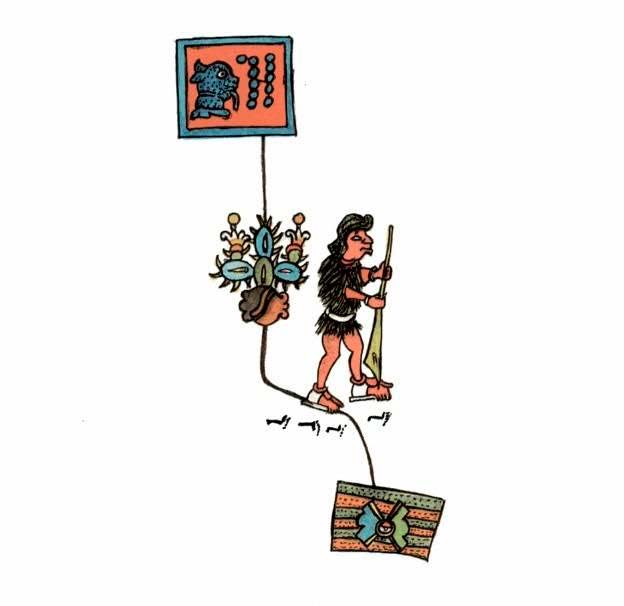
\includegraphics[width=1\textwidth]{images/codice.jpg}}}
  \end{center}
\end{figure}

The use of cartography to place the damage information also is useful not only to allocate resources in the aftermath of the disaster but also serves as historical evidence. In figure \cite{fig:quake1800} taken from \cite{AG3316} we can see the building that where damaged during an earthquake known as the *San Juan de Dios* earthquake \footnote{Back then the earthquakes where name acordingly to the day in which they happened.} that dates back to March 8, 1800, years before the Independence, during a age of economic and social prosperity.\\

Important earthquakes ocurred in the years 1845 and 1858 one of which is theorized to have been even stronger than the infamous earthquake of September 19, 1985. Paradoxically, these events that hit the state of Oaxaca pretty badly didn't produced as much damage as recent ones due to the lack of stablished cities in the state back then.

\begin{figure}[h]
  \begin{center}
    \subfigure{\label{fig:quake1800}\fbox{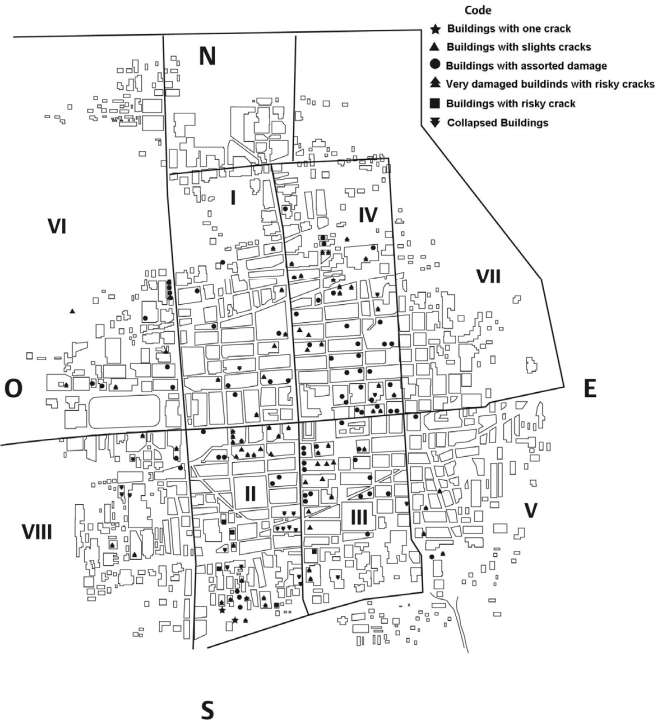
\includegraphics[width=1\textwidth]{images/quake1800.png}}}
  \end{center}
\end{figure}


\section{Objective}

It is a wondeful time to explore the use of novel technologies in all types of context. It is in human nature to create tools that revolutionize the way it modifies its envirmonment. We want to explore the use of Convolutional Neural Networks in the context of landcover classification. We believe that this field is very promising and will bloom even more in the comming years. 

\section{Scope}

It would be far too ambitious to cover every topic that is involved in the process of the classification using CNNs. We want to explain how do the networks work to a certain extent, but it is not in the scope of this work to untangle every single detail. In the same fashion, the field of Remote Sensing is far too big to be explored in this work. We assume a certain degree of knowledge in related topics and we expose some mathematical details in the appendix.\\

As we already mentioned, the field of Computer Vision is in its climax. Reviewing every single article that has been writen would be a daunting task. We offer a brief literature review that gives some context about the state-of-the art and we hope to build upon ideas and efforts done by a miryad of people. We aimed to built a system capable of procesing imagery and that could be deployed into a cluster for efficient computation.\\
